\documentclass[letterpaper,11pt]{article}
\usepackage{graphicx}
\usepackage{listings}
\usepackage[super]{nth}
\usepackage[hyphens]{url}
\usepackage{amsmath}
\usepackage[makeroom]{cancel}
\usepackage[table]{xcolor}
\usepackage{comment}
\usepackage[space]{grffile}

\lstset{
	basicstyle=\footnotesize,
	breaklines=true,
}

\begin{document}

\begin{titlepage}

\begin{center}

\Huge{Assignment 4}

\Large{CS 532:  Introduction to Web Science}

\Large{Spring 2016}

\Large{Manoj Chandra Kompalli}

\Large Finished on \today

\end{center}

\end{titlepage}

\newpage
\section*{1}

\subsection*{Question}

\begin{verbatim}
1.  Determine if the friendship paradox holds for my Facebook
account.* Compute the mean, standard deviation, and median of the
number of friends that my friends have.  Create a graph of the
number of friends (y-axis) and the friends themselves, sorted by
number of friends (x-axis).  (The friends don't need to be labeled
on the x-axis: just f1, f2, f3, ... fn.)  Do include me in the graph
and label me accordingly.

* = This used to be more interesting when you could more easily download
your friend's friends data from Facebook.  Facebook now requires each
friend to approve this operation, effectively making it impossible.

I will email to the list the XML file that contains my Facebook
friendship graph ca. Oct, 2013.  The interesting part of the file looks
like this (for 1 friend):

<node id="Johan_Bollen_1448621116">
        <data key="Label">Johan Bollen</data>
        <data key="uid"><![CDATA[1448621116]]></data>
        <data key="name"><![CDATA[Johan Bollen]]></data>
        <data key="mutual_friend_count"><![CDATA[37]]></data>
        <data key="friend_count"><![CDATA[420]]></data>
</node>

It is in GraphML format: http://graphml.graphdrawing.org/
\end{verbatim}

\newpage
\subsection*{Answer}
I was trying to figure out how to get my own graphml to fetch my friends data .I could not succeed due to facebook’s privacy settings. I have downloaded Dr. Nelson’s friend list in graphml format. Now the task ahead of me was to find a way to extract the graphml data and sort it.I researched and found a library called minidom which can extract the xml data. I have extracted the “data” tag and two key values name and friend count. The ``name`` got me all the friend’s names and friend\_count shown in Listing \ref{lst:q1codepy} gave me the count of friends for that friend.I have iterated the loop for all the friends to get the complete list. I have sorted the list in increasing order using Excel and copied the values to a text file.I had computed Dr. Nelson’s friend’s and added it to the list of his friends. 




I used the text file as input to R.I found the mean, median and standard deviation of the sorted list in R.Code shown in Listing \ref{lst:q1codeR}. I have plotted a bargraph shown in Figure \ref{fig:q1barplot} . I had found out that Dr. Nelson has less than half of the mean of his friends’ friends that is $154$ .This proves the friendship paradox.   

The R script generates these values:
\begin{lstlisting}[frame=single]

Mean   :358.987
Median :266.500
Std Dev:371.585

 
       
\end{lstlisting}
\begin{table}
\begin{tabular}{ l l }
\hline
\textbf{Mean} & 358.987 \\
\textbf{Median} & 266.500 \\
\textbf{Std Dev} & 371.585 \\
\hline
\end{tabular}
\caption{Statistics of Dr.Nelson's Friends' friends values taken from R}
\label{tab:q1statistics}
\end{table}

\clearpage
\begin{figure}[h]
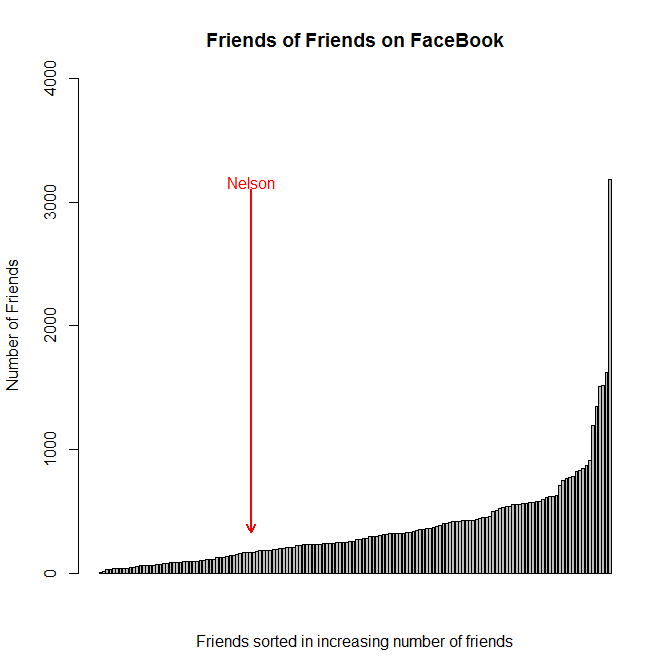
\includegraphics[scale=0.5]{qn1/Rgraphfinal.png}
\caption{Bar plot showing the count of Dr.Nelson's Facebook Friends' Friends}
\label{fig:q1barplot}
\end{figure}

\newpage
\lstinputlisting[language=Python,frame=single,caption={Python program for processing GraphML file },label=lst:q1codepy,captionpos=b,numbers=left,showspaces=false,showstringspaces=false,basicstyle=\footnotesize]{qn1/fbgraph.py}

\newpage
\lstinputlisting[language=R,frame=single,caption={R program for bar plot shown in Figure \ref{fig:q1barplot}},label=lst:q1codeR,captionpos=b,numbers=left,showspaces=false,showstringspaces=false,basicstyle=\footnotesize]{qn1/finalR.R}


\newpage
\section*{2}

\subsection*{Question}

\begin{verbatim}
2.  Determine if the friendship paradox holds for your Twitter account.
Since Twitter is a directed graph, use "followers" as value you measure
(i.e., "do your followers have more followers than you?").

Generate the same graph as in question #1, and calcuate the same 
mean, standard deviation, and median values.

For the Twitter 1.1 API to help gather this data, see:

https://dev.twitter.com/docs/api/1.1/get/followers/list

If you do not have followers on Twitter (or don't have more than 50),
then use my twitter account "phonedude_mln".


Extra credit, 3 points:
\end{verbatim}

\newpage
\subsection*{Answer}
Again, a similar question but a different approach. I had used Tweepy API to extract links in the previous assignments. Thankfully, this experience came in handy. It was a relatively simple task this time. 
I had to use tweepy.Cursor object and followers\_count gave me the number of followers of my followers. screen\_name gave me the user name .I have again looped through all users and wrote the values to a csv file. I had  sorted the csv file,copied it to a text file and extracted the data.
I used this list to generate the mean, median and standard deviation. This time around, the mean was even higher due to a single user having large number of followers. I have plotted a bar graph  which again puts me nowhere in comparision to the mean. Friendship paradox is proved again.





From the output, I can see that I have $34$ followers.It is greater than the median.It means that I have a considerable rank amongst my followers. The R script shown in Listing \ref{lst:q2codeR} creates a similar bar plot to that shown in answer one and produces the statistics shown in listing \ref{tab:q2statistics}.

\begin{lstlisting}[frame=single]
Mean:  141518.205
Median:  25
Std Dev:  824927.542

     
\end{lstlisting}


\begin{table}
\begin{tabular}{ l l }
\hline
\textbf{Mean} & 141518.205 \\
\textbf{Median} &  25 \\
\textbf{Std Dev} & 824927.542 \\
\hline
\end{tabular}
\caption{Statistics on the count of my Twitter followers' followers, values straight from R}
\label{tab:q2statistics}
\end{table}

\clearpage
\begin{figure}[h]
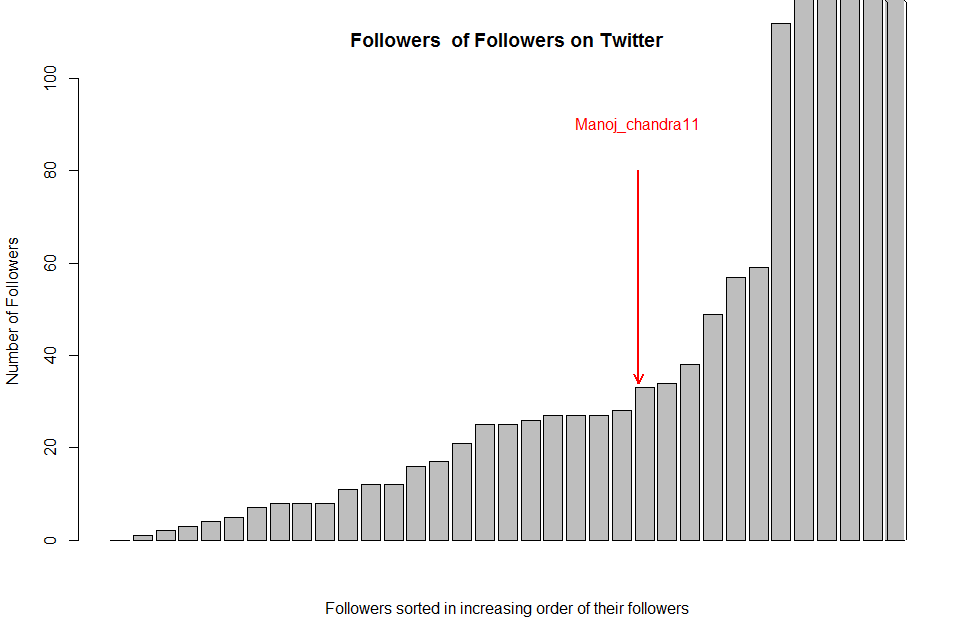
\includegraphics[scale=0.35]{qn2/Rimage.png}
\caption{Bar plot showing the count of my Twitter followers' followers}
\label{fig:q2barplot}
\end{figure}


\newpage
\lstinputlisting[language=Python,frame=single,caption={Python program for acquiring Twitter followers for phonedude\_mln},label=lst:q2codepy,captionpos=b,numbers=left,showspaces=false,showstringspaces=false,basicstyle=\footnotesize]{qn2/followers.py}

\newpage
\lstinputlisting[language=R,frame=single,caption={R program for bar plot shown in Figure \ref{fig:q2barplot}},label=lst:q2codeR,captionpos=b,numbers=left,showspaces=false,showstringspaces=false,basicstyle=\footnotesize]{qn2/Rcommands.R}




\newpage
\section*{3}

\subsection*{Question}

\begin{verbatim}
3.  Repeat question #1, but with your LinkedIn profile.
\end{verbatim}

\newpage
\subsection*{Answer}

Not attempted.

\newpage
\section*{4}

\subsection*{Question}

\begin{verbatim}
Extra credit, 1 point:

4.  Repeat question #2, but change "followers" to "following"?  In
other words, are the people I am following following more people?
\end{verbatim}

\newpage
\subsection*{Answer}
This is again a very similar approach to what I did with the second question.I had to extract the friends’ friends data. It is the ``following`` data. Here, I used friends\_count instead of followers\_count.    

The result appears to hold in the case of ``following'', as shown in Figure \ref{fig:q4barplot}.I again lose terribly to the mean value.Hence,friendship paradox is proved again.  The Python code for this case is in Listing \ref{lst:q4codepy} and the R code for this Figure is in Listing \ref{lst:q4codeR}.  The statistics are shown in Table \ref{tab:q4statistics}.

Both scripts are executed as shown in the answer to Question 2.

\begin{table}
\begin{tabular}{ l l }
\hline
\textbf{Mean} & 4938.863 \\
\textbf{Median} & 115 \\
\textbf{Std Dev} &  2881.577 \\
\hline
\end{tabular}
\caption{Statistics on the count of my Twitter friends' friends, values straight from R}
\label{tab:q4statistics}
\end{table}

\clearpage
\begin{figure}[h]
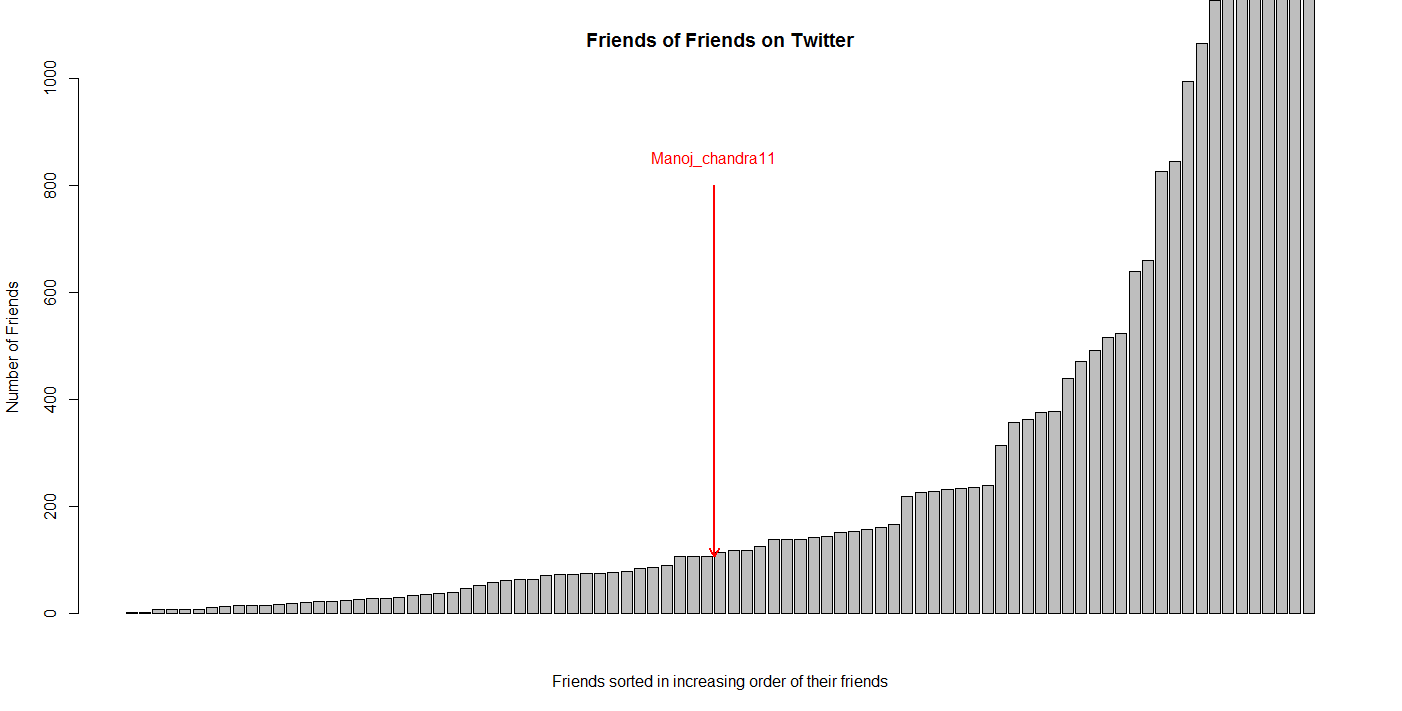
\includegraphics[scale=0.3]{qn4/RGraph.png}
\caption{Bar plot showing the count of my Twitter friends' friends}
\label{fig:q4barplot}
\end{figure}


\newpage
\lstinputlisting[language=Python,frame=single,caption={Python program for acquiring my Twitter followers},label=lst:q4codepy,captionpos=b,numbers=left,showspaces=false,showstringspaces=false,basicstyle=\footnotesize]{qn4/following.py}

\newpage
\lstinputlisting[language=R,frame=single,caption={R program for bar plot shown in Figure \ref{fig:q4barplot}},label=lst:q4codeR,captionpos=b,numbers=left,showspaces=false,showstringspaces=false,basicstyle=\footnotesize]{qn4/Rcommands.R}



\clearpage
\bibliographystyle{acm}
\bibliography{references}

\end{document}